% ==============================================================================
% Imscribing Grammar — TikZ Figures for Publication-Quality Manuscript
% Author: Lando ⊗ ⊙perator
% Five diagrams: Crystal Lattice, B4 Bilattice, Gene Pipeline, Serpent Rod, CLINK
% Compile: lualatex figures_tikz.tex
% ==============================================================================
\documentclass[border=8pt,multi=tikzpicture]{standalone}
\usepackage{fontspec}
\usepackage{tikz}
\usepackage{amsmath,amssymb}
\usepackage{xcolor}

\usetikzlibrary{
  arrows.meta,
  positioning,
  shapes.geometric,
  shapes.multipart,
  fit,
  backgrounds,
  calc,
  chains,
  decorations.pathreplacing,
  decorations.markings,
}

% ── Color palette (RGB, no HSB) ──
\definecolor{Dfamily}{RGB}{46,134,171}     % blue — evaluator primitives
\definecolor{Tfamily}{RGB}{162,59,114}     % plum — topological primitives
\definecolor{Pfamily}{RGB}{241,143,1}      % amber — parity primitives
\definecolor{B4top}{RGB}{75,0,130}         % indigo — Both
\definecolor{B4true}{RGB}{46,125,50}       % green — True
\definecolor{B4false}{RGB}{198,40,40}      % red — False
\definecolor{B4bot}{RGB}{84,110,122}       % blue-grey — Neither
\definecolor{stagebg}{RGB}{236,239,241}    % light grey — stage boxes
\definecolor{arrowcol}{RGB}{55,71,79}      % dark grey — arrows
\definecolor{frob}{RGB}{123,31,162}        % purple — Frobenius highlight

% ── 9-layer gradient colors (RGB, violet→amber) ──
\definecolor{layer0}{RGB}{120,25,145}
\definecolor{layer1}{RGB}{100,40,170}
\definecolor{layer2}{RGB}{70,65,195}
\definecolor{layer3}{RGB}{40,95,210}
\definecolor{layer4}{RGB}{20,130,190}
\definecolor{layer5}{RGB}{20,160,145}
\definecolor{layer6}{RGB}{60,185,95}
\definecolor{layer7}{RGB}{130,200,50}
\definecolor{layer8}{RGB}{210,180,20}

% ── Shared styles ──
\tikzset{
  primnode/.style={
    circle, draw, thick, minimum size=2.2em,
    font=\bfseries, inner sep=1pt
  },
  Dnode/.style={primnode, fill=Dfamily!15, draw=Dfamily!70!black, text=Dfamily!80!black},
  Tnode/.style={primnode, fill=Tfamily!15, draw=Tfamily!70!black, text=Tfamily!80!black},
  Pnode/.style={primnode, fill=Pfamily!15, draw=Pfamily!70!black, text=Pfamily!80!black},
  dualedge/.style={thick, frob!50, >=Stealth, <->},
  vertedge/.style={thick, frob!30},
  stagebox/.style={
    rectangle, draw=arrowcol!60, fill=stagebg, rounded corners=4pt,
    text width=12.5cm, align=left, font=\footnotesize,
    minimum height=2.4em, inner sep=6pt
  },
  bigarrow/.style={->, >=Stealth, thick, arrowcol!70},
  smallarrow/.style={->, >=Stealth, semithick, arrowcol!60},
  layerbox/.style={
    rectangle, draw=arrowcol!50, fill=white, rounded corners=3pt,
    text width=11.5cm, align=left, font=\footnotesize,
    minimum height=2.0em, inner sep=5pt
  },
  b4node/.style={
    circle, draw, very thick, minimum size=3.0em,
    font=\bfseries\Large, inner sep=0pt
  },
  enginebox/.style={
    rectangle, draw=arrowcol!70, fill=stagebg, rounded corners=5pt,
    text width=9.5cm, align=center, font=\footnotesize,
    minimum height=3.0em, inner sep=8pt
  },
}

\begin{document}

% ══════════════════════════════════════════════════════════════════════════════
% FIGURE 1: The 12-Primitive Crystal Lattice
% ══════════════════════════════════════════════════════════════════════════════
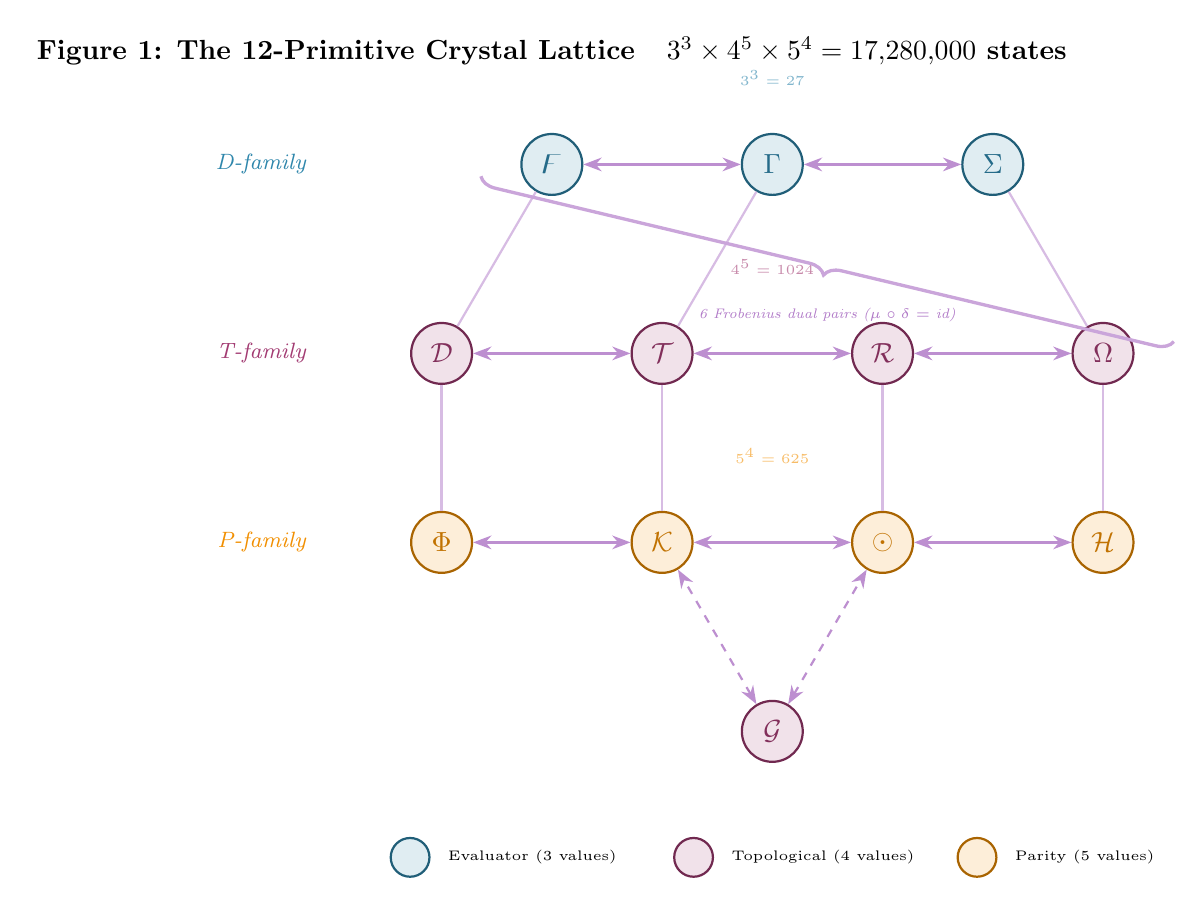
\begin{tikzpicture}[node distance=2.4cm and 2.8cm]

  % ── Row 1: D-family (evaluators) ──
  \node[Dnode] (F)  at (0,    6.0) {$\digamma$};
  \node[Dnode] (G)  at (2.8,  6.0) {$\Gamma$};
  \node[Dnode] (S)  at (5.6,  6.0) {$\Sigma$};

  % ── Row 2: T-family bridge layer ──
  \node[Tnode] (D)  at (-1.4, 3.6) {$\mathcal{D}$};
  \node[Tnode] (T)  at (1.4,  3.6) {$\mathcal{T}$};
  \node[Tnode] (R)  at (4.2,  3.6) {$\mathcal{R}$};
  \node[Tnode] (O)  at (7.0,  3.6) {$\Omega$};

  % ── Row 3: P-family (parity) ──
  \node[Pnode] (Ph) at (-1.4, 1.2) {$\Phi$};
  \node[Pnode] (K)  at (1.4,  1.2) {$\mathcal{K}$};
  \node[Pnode] (Cr) at (4.2,  1.2) {$\odot$};
  \node[Pnode] (H)  at (7.0,  1.2) {$\mathcal{H}$};

  % ── Row 4: Composition bridge ──
  \node[Tnode] (Gm) at (2.8,  -1.2) {$\mathcal{G}$};

  % ── Family background labels ──
  \node[font=\footnotesize\itshape, text=Dfamily, anchor=east] at (-3.0, 6.0) {D-family};
  \node[font=\footnotesize\itshape, text=Tfamily, anchor=east] at (-3.0, 3.6) {T-family};
  \node[font=\footnotesize\itshape, text=Pfamily, anchor=east] at (-3.0, 1.2) {P-family};

  % ── Family cardinality annotations ──
  \node[font=\tiny, text=Dfamily!60]  at (2.8, 7.1)  {$3^3 = 27$};
  \node[font=\tiny, text=Tfamily!60]  at (2.8, 4.7)  {$4^5 = 1024$};
  \node[font=\tiny, text=Pfamily!60]  at (2.8, 2.3)  {$5^4 = 625$};

  % ── Horizontal edges (intra-family) ──
  \draw[dualedge] (F)  -- (G);
  \draw[dualedge] (G)  -- (S);
  \draw[dualedge] (D)  -- (T);
  \draw[dualedge] (T)  -- (R);
  \draw[dualedge] (R)  -- (O);
  \draw[dualedge] (Ph) -- (K);
  \draw[dualedge] (K)  -- (Cr);
  \draw[dualedge] (Cr) -- (H);

  % ── Vertical edges (inter-family) ──
  \draw[vertedge] (F)  -- (D);
  \draw[vertedge] (G)  -- (T);
  \draw[vertedge] (S)  -- (O);
  \draw[vertedge] (D)  -- (Ph);
  \draw[vertedge] (T)  -- (K);
  \draw[vertedge] (R)  -- (Cr);
  \draw[vertedge] (O)  -- (H);

  % ── Bridge edges from Gm → K, Cr ──
  \draw[dualedge, dashed] (Gm) -- (K);
  \draw[dualedge, dashed] (Gm) -- (Cr);

  % ── Frobenius dual-pair bracket ──
  \draw [decorate, decoration={brace, amplitude=6pt, mirror}, frob!40, very thick]
    ($(F.west)  + (-0.5,-0.15)$) -- ($(O.east)  + (0.5,0.15)$)
    node [midway, below=14pt, font=\tiny\itshape, text=frob!60] {6 Frobenius dual pairs ($\mu\circ\delta = \text{id}$)};

  % ── Title ──
  \node[font=\bfseries, above=0.6cm of F, yshift=4pt]
    {Figure 1: The 12-Primitive Crystal Lattice\quad $3^3 \times 4^5 \times 5^4 = 17{,}280{,}000$ states};

  % ── Legend ──
  \node[Dnode, minimum size=1.4em, font=\tiny] (legD) at (-1.8, -2.8) {};
  \node[right=0.1cm of legD, font=\tiny] {Evaluator (3 values)};
  \node[Tnode, minimum size=1.4em, font=\tiny] (legT) at (1.8, -2.8) {};
  \node[right=0.1cm of legT, font=\tiny] {Topological (4 values)};
  \node[Pnode, minimum size=1.4em, font=\tiny] (legP) at (5.4, -2.8) {};
  \node[right=0.1cm of legP, font=\tiny] {Parity (5 values)};

\end{tikzpicture}

% ══════════════════════════════════════════════════════════════════════════════
% FIGURE 2: The Belnap FOUR Bilattice
% ══════════════════════════════════════════════════════════════════════════════
\begin{tikzpicture}

  % ── Nodes ──
  \node[b4node, fill=B4top!15,   draw=B4top!80,   text=B4top!80]   (B) at (0,  4)   {$\mathbf{B}$};
  \node[b4node, fill=B4true!15,  draw=B4true!80,  text=B4true!80]  (T) at (-2.4, 1.5) {$\mathbf{T}$};
  \node[b4node, fill=B4false!15, draw=B4false!80, text=B4false!80] (F) at (2.4,  1.5) {$\mathbf{F}$};
  \node[b4node, fill=B4bot!15,   draw=B4bot!80,   text=B4bot!80]   (N) at (0, -1)   {$\mathbf{N}$};

  % ── Edges ──
  \draw[>=Stealth, <->, very thick, B4top!40]   (B) -- (T);
  \draw[>=Stealth, <->, very thick, B4top!40]   (B) -- (F);
  \draw[>=Stealth, <->, very thick, B4bot!40]   (T) -- (N);
  \draw[>=Stealth, <->, very thick, B4bot!40]   (F) -- (N);

  % ── Annotations ──
  \node[font=\small\itshape, right=0.8cm of B] {Both: $\{t,f\}$};
  \node[font=\small\itshape, left=0.8cm of T]  {True: $\{t\}$};
  \node[font=\small\itshape, right=0.8cm of F] {False: $\{f\}$};
  \node[font=\small\itshape, below=0.5cm of N] {Neither: $\varnothing$};

  % ── Order labels ──
  \node[font=\footnotesize, rotate=90, text=B4top!50, anchor=south]
    at (-4.4, 2.75) {Information order $\leq_i$: $\mathbf{N} \to \{\mathbf{T},\mathbf{F}\} \to \mathbf{B}$};
  \node[font=\footnotesize, text=B4bot!50, anchor=west]
    at (3.5, 1.5) {Truth order $\leq_t$: $\mathbf{F} \to \{\mathbf{N},\mathbf{B}\} \to \mathbf{T}$};

  % ── B₄ in genetics inset ──
  \begin{scope}[shift={(6.0, 3.5)}]
    \node[font=\bfseries\footnotesize, anchor=west] at (0, 0.5) {Nucleotide $\to$ B₄};
    \draw[gray!40] (-0.2, 0.1) -- (4.5, 0.1);
    \node[font=\tiny, anchor=west] at (0, -0.3)  {A (Adenine)     $\to \mathbf{T}$};
    \node[font=\tiny, anchor=west] at (0, -0.75) {U/T (Ura/Thy)   $\to \mathbf{F}$};
    \node[font=\tiny, anchor=west] at (0, -1.2)  {G (Guanine)     $\to \mathbf{B}$};
    \node[font=\tiny, anchor=west] at (0, -1.65) {C (Cytosine)    $\to \mathbf{N}$};
    \draw[gray!40] (-0.2, -1.9) -- (4.5, -1.9);
    \node[font=\tiny\itshape, text=frob!70, anchor=west] at (0, -2.3)
      {B₄\textsuperscript{3} = 64 codons};
  \end{scope}

  % ── Title ──
  \node[font=\bfseries, above=0.6cm of B, yshift=6pt]
    {Figure 2: The Belnap FOUR Bilattice — Paraconsistent Kernel};

\end{tikzpicture}

% ══════════════════════════════════════════════════════════════════════════════
% FIGURE 3: The 7-Stage Gene → Protein Pipeline
% ══════════════════════════════════════════════════════════════════════════════
\begin{tikzpicture}[node distance=0.75cm]

  % ── Stage boxes ──
  \node[stagebox] (S0) {
    \textbf{Stage 0: DNA GENE}
    \hfill {\small D:tri\quad T:$\sqcap$\quad R:$\leftrightarrow$\quad $\Phi$:$\sim$\quad F:$\ell$\quad K:slow\quad $\Gamma$:$\beth$\quad G:$\blacktriangleright$\quad $\odot$:$<$c\quad H:$\circlearrowright\circlearrowright$\quad $\Sigma$:1\quad $\Omega$:$\mathbb{Z}$}
  };
  \node[stagebox, below=of S0] (S1) {
    \textbf{Stage 1: PRE-mRNA}
    \hfill {\small D:tri\quad T:$\subset$\quad R:$\to$\quad $\Phi$:$\varnothing$\quad F:$\ell$\quad K:mod\quad $\Gamma$:$\beth$\quad G:$\blacktriangleright$\quad $\odot$:$<$c\quad H:$\circlearrowright$\quad $\Sigma$:1\quad $\Omega$:0}
  };
  \node[stagebox, below=of S1] (S2) {
    \textbf{Stage 2: MATURE mRNA}
    \hfill {\small D:tri\quad T:$\subset$\quad R:$\dagger$\quad $\Phi$:$\varnothing$\quad F:$\ell$\quad K:slow\quad $\Gamma$:$\beth$\quad G:$\blacktriangleright$\quad $\odot$:$<$c\quad H:$\circlearrowright$\quad $\Sigma$:1\quad $\Omega$:0}
  };
  \node[stagebox, below=of S2] (S3) {
    \textbf{Stage 3: NASCENT POLYPEPTIDE}
    \hfill {\small D:tri\quad T:$\bowtie$\quad R:$\to$\quad $\Phi$:$\varnothing$\quad F:$\ell$\quad K:fast\quad $\Gamma$:$\beth$\quad G:$\blacktriangleright$\quad $\odot$:$<$c\quad H:$\circlearrowright\circlearrowright$\quad $\Sigma$:$\neq$\quad $\Omega$:0}
  };
  \node[stagebox, below=of S3] (S4) {
    \textbf{Stage 4: SECONDARY STRUCTURE}
    \hfill {\small D:$\odot$\quad T:$\odot$\quad R:$\dagger$\quad $\Phi$:$\sim$\quad F:$\ell$\quad K:mod\quad $\Gamma$:$\beth$\quad G:$\blacktriangleright$\quad $\odot$:$<$c\quad H:$\circlearrowright\circlearrowright$\quad $\Sigma$:n\quad $\Omega$:0}
  };
  \node[stagebox, below=of S4] (S5) {
    \textbf{Stage 5: TERTIARY STRUCTURE}
    \hfill {\small D:$\odot$\quad T:$\odot$\quad R:$\leftrightarrow$\quad $\Phi$:$\varnothing$\quad F:$\ell$\quad K:slow\quad $\Gamma$:$\aleph$\quad G:$\wedge$\quad $\odot$:$<$c\quad H:$\circlearrowright\circlearrowright$\quad $\Sigma$:1\quad $\Omega$:0}
  };
  \node[stagebox, below=of S5] (S6) {
    \textbf{Stage 6: QUATERNARY STRUCTURE}
    \hfill {\small D:$\odot$\quad T:$\odot$\quad R:$\leftrightarrow$\quad $\Phi$:$\sim$\quad F:$\ell$\quad K:slow\quad $\Gamma$:$\beth$\quad G:$\wedge$\quad $\odot$:$<$c\quad H:$\circlearrowright$\quad $\Sigma$:$\neq$\quad $\Omega$:$\mathbb{Z}$}
  };

  % ── Arrows with transition labels ──
  \draw[bigarrow] (S0.south) -- (S1.north)
    node[midway, right=0.3cm, font=\tiny\itshape, align=left, text=arrowcol!80]
      {transcription\\T:$\sqcap$$\to$$\subset$, R:$\leftrightarrow$$\to$$\to$\\K:slow$\to$mod, $\Omega$:$\mathbb{Z}$$\to$0};
  \draw[bigarrow] (S1.south) -- (S2.north)
    node[midway, right=0.3cm, font=\tiny\itshape, text=arrowcol!80]
      {splicing \quad R:$\to$$\to$$\dagger$};
  \draw[bigarrow] (S2.south) -- (S3.north)
    node[midway, right=0.3cm, font=\tiny\itshape, align=left, text=arrowcol!80]
      {translation\\R:$\dagger$$\to$$\to$, K:slow$\to$fast\\H:$\circlearrowright$$\to$$\circlearrowright\circlearrowright$, $\Sigma$:1$\to$$\neq$};
  \draw[bigarrow] (S3.south) -- (S4.north)
    node[midway, right=0.3cm, font=\tiny\itshape, align=left, text=arrowcol!80]
      {folding I (collapse)\\D:tri$\to$$\odot$, T:$\bowtie$$\to$$\odot$\\$\Phi$:$\varnothing$$\to$$\sim$, $\Sigma$:$\neq$$\to$n};
  \draw[bigarrow] (S4.south) -- (S5.north)
    node[midway, right=0.3cm, font=\tiny\itshape, align=left, text=arrowcol!80]
      {folding II (packing)\\R:$\dagger$$\to$$\leftrightarrow$, $\Gamma$:$\beth$$\to$$\aleph$\\G:$\blacktriangleright$$\to$$\wedge$, $\Sigma$:n$\to$1};
  \draw[bigarrow] (S5.south) -- (S6.north)
    node[midway, right=0.3cm, font=\tiny\itshape, align=left, text=arrowcol!80]
      {assembly\\$\Phi$:$\varnothing$$\to$$\sim$, H:$\circlearrowright\circlearrowright$$\to$$\circlearrowright$\\$\Sigma$:1$\to$$\neq$, $\Omega$:0$\to$$\mathbb{Z}$};

  % ── B₄ flow annotation ──
  \node[font=\tiny\itshape, text=frob!70, anchor=east] at ($(S0.west) + (-0.3, 0.3)$)
    {B₄ flow: N $\to$ T $\to$ B $\to$ F $\to$ T $\to$ T};

  % ── Closure bracket ──
  \draw [decorate, decoration={brace, amplitude=10pt}, frob!40, very thick]
    ($(S0.north west) + (-0.2, 0.3)$) -- ($(S6.south west) + (-0.2, -0.3)$)
    node [midway, left=18pt, font=\tiny\itshape, text=frob!60, rotate=90]
      {$\Delta$(DNA, Quaternary) = 4.0};

  % ── Title ──
  \node[font=\bfseries, above=0.5cm of S0, yshift=4pt]
    {Figure 3: The 7-Stage Gene $\to$ Protein Pipeline with Primitive Transitions};

\end{tikzpicture}

% ══════════════════════════════════════════════════════════════════════════════
% FIGURE 4: The Serpent Rod Folding Engine
% ══════════════════════════════════════════════════════════════════════════════
\begin{tikzpicture}[node distance=0.7cm]

  % ── Input ──
  \node[font=\small\ttfamily, align=center] (input)
    {\textbf{Input:} DNA/RNA Sequence \texttt{AUG UGG UGC UAC UUU AUU CAC ...}};

  % ── Engine boxes ──
  \node[enginebox, below=of input] (b4eval) {
    \textbf{1. B₄ EVALUATION}\\[2pt]
    {\footnotesize Nucleotide $\to$ B₄: A$\to$T, U$\to$F, G$\to$B, C$\to$N}\\[1pt]
    {\footnotesize Codon triplets $\to$ B₄ winding path (B₄\textsuperscript{3} = 64 states)}
  };

  \node[enginebox, below=of b4eval] (rama) {
    \textbf{2. B₄ $\to$ RAMACHANDRAN MAPPING}\\[2pt]
    {\footnotesize Transition $(b_i, b_{i+1}) \to (\phi, \psi)$ per residue}\\[1pt]
    {\footnotesize 16 B₄ transition types $\to$ 4 secondary structure classes}
  };

  \node[enginebox, below=of rama] (backbone) {
    \textbf{3. 3D BACKBONE RECONSTRUCTION}\\[2pt]
    {\footnotesize Internal $\to$ Cartesian: place\_atom algorithm}\\[1pt]
    {\footnotesize N, C$\alpha$, C, O per residue (bond lengths/angles from Pauling 1951)}
  };

  \node[enginebox, below=of backbone] (energy) {
    \textbf{4. CONTACT PREDICTION + ENERGY}\\[2pt]
    {\footnotesize C$\alpha$--C$\alpha$ $<$ 8\,\AA\ contacts \quad $E = E_{\text{LJ}} + E_{\text{HB}} + E_{\text{elec}}$}\\[1pt]
    {\footnotesize Primitive activation: 6--10 of 12 \quad $\mu\circ\delta = \text{id}$ verified}
  };

  % ── Output ──
  \node[font=\small\bfseries, below=of energy, fill=frob!10, draw=frob!40, rounded corners=3pt,
        minimum width=9.5cm, minimum height=1.6em, inner sep=6pt, align=center]
    (output) {\textbf{Output:} PDB Structure File (v3.3)};

  % ── Arrows ──
  \draw[bigarrow] (input.south)    -- (b4eval.north);
  \draw[bigarrow] (b4eval.south)   -- (rama.north);
  \draw[bigarrow] (rama.south)     -- (backbone.north);
  \draw[bigarrow] (backbone.south) -- (energy.north);
  \draw[bigarrow] (energy.south)   -- (output.north);

  % ── Side annotations ──
  \node[font=\tiny\itshape, text=Tfamily!80, anchor=west]
    at ($(b4eval.east) + (0.3, 0.0)$) {16 transition pairs};

  \node[font=\tiny\itshape, text=Pfamily!80, anchor=west]
    at ($(rama.east) + (0.3, 0.0)$) {$(\phi,\psi)$ basins};

  \node[font=\tiny\itshape, text=Dfamily!80, anchor=west]
    at ($(backbone.east) + (0.3, 0.0)$) {N--C$\alpha$--C geometry};

  \node[font=\tiny\itshape, text=frob!80, anchor=west]
    at ($(energy.east) + (0.3, 0.0)$) {Frobenius closed};

  % ── Ramachandran inset ──
  \begin{scope}[shift={(6.8, 1.8)}]
    \draw[->, thin] (-1.5,0) -- (1.8,0) node[right, font=\tiny] {$\phi$};
    \draw[->, thin] (0,-1.2) -- (0,1.2) node[above, font=\tiny] {$\psi$};
    % alpha-helix basin
    \draw[fill=B4true!30, draw=B4true!60, thick, rounded corners=2pt]
      (-1.0,0.7) ellipse (0.35 and 0.3);
    \node[font=\tiny\bfseries, text=B4true!80] at (-1.0,1.15) {$\alpha$};
    % beta-sheet basin
    \draw[fill=B4top!30, draw=B4top!60, thick, rounded corners=2pt]
      (0.6,-0.4) ellipse (0.5 and 0.45);
    \node[font=\tiny\bfseries, text=B4top!80] at (0.6,-0.05) {$\beta$};
    % left-handed helix
    \draw[fill=B4false!20, draw=B4false!60, thick, rounded corners=2pt]
      (0.9,0.5) ellipse (0.25 and 0.2);
    \node[font=\tiny\bfseries, text=B4false!80] at (0.9,0.85) {$\alpha_L$};
    \node[font=\tiny, below=0.3cm, text=arrowcol!60] {Ramachandran map};
  \end{scope}

  % ── Title ──
  \node[font=\bfseries, above=0.5cm of input, yshift=2pt]
    {Figure 4: The Serpent Rod Folding Engine — B₄ $\to$ Ramachandran $\to$ 3D Backbone $\to$ PDB};

\end{tikzpicture}

% ══════════════════════════════════════════════════════════════════════════════
% FIGURE 5: The CLINK L0→L8 Whole-Organism Chain
% ══════════════════════════════════════════════════════════════════════════════
\begin{tikzpicture}[node distance=0.55cm]

  % ── Layer 0: Quark Color Confinement ──
  \node[layerbox, fill=layer0!12, draw=layer0!60] (L0) at (0, 10.0) {
    \textbf{L0: QUARK COLOR CONFINEMENT}
    \hfill {\footnotesize\itshape SU(3) gauge, 3-color singlets}
    \hfill {\footnotesize $\Omega$:$\mathbb{Z}$, $\Sigma$:1 \quad|\quad B₄: $\mathbf{T}$}
  };

  % ── Layer 1: Nuclear Force ──
  \node[layerbox, fill=layer1!12, draw=layer1!60, below=of L0] (L1) {
    \textbf{L1: NUCLEAR FORCE}
    \hfill {\footnotesize\itshape Residual strong, pion exchange}
    \hfill {\footnotesize $\Omega$:0, $\Sigma$:n \quad|\quad B₄: $\mathbf{B}$}
  };

  % ── Layer 2: Atomic Electron Structure ──
  \node[layerbox, fill=layer2!12, draw=layer2!60, below=of L1] (L2) {
    \textbf{L2: ATOMIC ELECTRON STRUCTURE}
    \hfill {\footnotesize\itshape QED, orbitals, Pauli exclusion}
    \hfill {\footnotesize $\Omega$:0, $\Sigma$:1 \quad|\quad B₄: $\mathbf{T}$}
  };

  % ── Layer 3: Molecular Bonding ──
  \node[layerbox, fill=layer3!12, draw=layer3!60, below=of L2] (L3) {
    \textbf{L3: MOLECULAR BONDING}
    \hfill {\footnotesize\itshape Covalent/ionic, H-bond networks}
    \hfill {\footnotesize $\Omega$:0, $\Sigma$:$\neq$ \quad|\quad B₄: $\mathbf{T}$}
  };

  % ── Layer 4: Biomolecule Assembly ──
  \node[layerbox, fill=layer4!12, draw=layer4!60, below=of L3] (L4) {
    \textbf{L4: BIOMOLECULE ASSEMBLY}
    \hfill {\footnotesize\itshape DNA, RNA, proteins, lipids}
    \hfill {\footnotesize $\Omega$:0, $\Sigma$:n \quad|\quad B₄: $\mathbf{B}$}
  };

  % ── Layer 5: Cellular Compartments ──
  \node[layerbox, fill=layer5!12, draw=layer5!60, below=of L4] (L5) {
    \textbf{L5: CELLULAR COMPARTMENTALIZATION}
    \hfill {\footnotesize\itshape Membranes, organelles, cytosol}
    \hfill {\footnotesize $\Omega$:0, $\Sigma$:$\neq$ \quad|\quad B₄: $\mathbf{B}$}
  };

  % ── Layer 6: Tissue Morphogenesis ──
  \node[layerbox, fill=layer6!12, draw=layer6!60, below=of L5] (L6) {
    \textbf{L6: TISSUE MORPHOGENESIS}
    \hfill {\footnotesize\itshape Cell adhesion, ECM, patterning}
    \hfill {\footnotesize $\Omega$:$\mathbb{Z}_2$, $\Sigma$:$\neq$ \quad|\quad B₄: $\mathbf{B}$}
  };

  % ── Layer 7: Organogenesis ──
  \node[layerbox, fill=layer7!12, draw=layer7!60, below=of L6] (L7) {
    \textbf{L7: ORGANOGENESIS}
    \hfill {\footnotesize\itshape Organ primordia, vascularization}
    \hfill {\footnotesize $\Omega$:$\mathbb{Z}$, $\Sigma$:$\neq$ \quad|\quad B₄: $\mathbf{B}$}
  };

  % ── Layer 8: Whole-Organism Integration ──
  \node[layerbox, fill=layer8!12, draw=layer8!60, below=of L7] (L8) {
    \textbf{L8: WHOLE-ORGANISM INTEGRATION}
    \hfill {\footnotesize\itshape Nervous, endocrine, immune networks}
    \hfill {\footnotesize $\Omega$:NA, $\Sigma$:$\neq$ \quad|\quad B₄: $\mathbf{B}$}
  };

  % ── Connector arrows ──
  \foreach \i in {1,...,8} {
    \pgfmathtruncatemacro{\prev}{\i-1}
    \draw[smallarrow, layer\i!40] (L\prev.south) -- (L\i.north);
  }

  % ── Promotion pathway bracket ──
  \draw [decorate, decoration={brace, amplitude=8pt, mirror}, frob!40, thick]
    ($(L8.south east) + (0.2, -0.3)$) -- ($(L5.north east) + (0.2, 0.3)$)
    node [midway, right=10pt, font=\tiny\itshape, text=frob!60, align=left]
      {Promotion\\pathway\\ZFC $\to$ ZFC$_t$ $\to$ ZFC$_{fe}$\\$\to$ CLINK L8};

  % ── Winding progression arrow (right side) ──
  \draw[>=Stealth, ->, thick, frob!25]
    ($(L0.north east) + (2.8, -0.2)$) -- ($(L8.south east) + (2.8, 0.2)$)
    node[midway, right=0.2cm, font=\tiny\itshape, text=frob!50, rotate=90]
      {$\Omega$: $\mathbb{Z} \to 0 \to \mathbb{Z}_2 \to \mathbb{Z} \to$ NA};

  % ── Layer4 Designer highlight ──
  \draw[thick, frob!50, dashed, rounded corners=3pt]
    ($(L4.north west) + (-0.15, 0.15)$) rectangle ($(L4.south east) + (0.15, -0.15)$);
  \node[font=\tiny\bfseries, text=frob!70, anchor=west] at ($(L4.east) + (0.5, 0.0)$)
    {$\leftarrow$ Layer4 Designer};
  \node[font=\tiny\itshape, text=frob!50, anchor=west] at ($(L4.east) + (0.5, -0.35)$)
    {(Gene $\to$ Protein $\to$ PDB)};

  % ── Frobenius invariant annotation ──
  \node[font=\tiny\itshape, text=frob!50, anchor=east] at ($(L0.west) + (-0.3, 0.3)$)
    {$\mu\circ\delta = \text{id}$};

  % ── Title ──
  \node[font=\bfseries, above=0.5cm of L0, yshift=2pt]
    {Figure 5: The CLINK L0$\to$L8 Whole-Organism Design Chain};

\end{tikzpicture}

\end{document}
